\chapter{Command Line Interfaces}

\section{\pointmatching}
\label{sec:example:pointmatching}

We exemplify here the use of \pointmatching to generate a vector field with two pairings $\{ 
(35,35,0) \rightarrow (60,40,0),
(65,60,0) \rightarrow (40,65,0) \}$, the first points being in the floating image while the second ones are in the reference image (see figure \ref{fig:exe:pointmatching:1}).

Test images can be generated with the following commands. 
\begin{code}{1}
\% createGrid -dim 100 100 mosaic.mha -type mosaic -spacing 10 10 \\
\% createGrid -dim 100 100 grid.mha -spacing 10 10
copy -norma mosaic.mha mosaic.mha
\end{code}

\begin{figure}[ht]
\begin{center}
\begin{tabular}{cc}
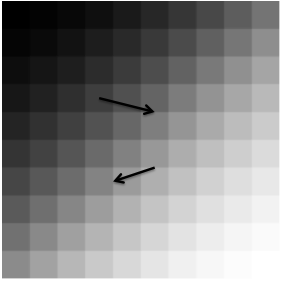
\includegraphics[width=35mm]{use-examples/pointmatching/figures/pairings.png} &
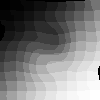
\includegraphics[width=35mm]{use-examples/pointmatching/mosaic-10-10-05.png} \\
&
$(d_p, d_f, \sigma_f) = (10,10,5)$
\end{tabular}
\end{center}
\caption{\label{fig:exe:pointmatching:1} The two pairings superimposed on a mosaic test image, and the resampled image with the deformation computed with $(d_p, d_f, \sigma_f) = (10,10,5)$.}
\end{figure}

The options passed to \pointmatching will be
\begin{code}{1}
-vector-propagation-distance $d_p$
-vector-fading-distance $d_f$
-fluid-sigma $\sigma_f$
\end{code}
where $d_p$, $d_f$, and $\sigma_f$ denotes respectively the propagation distance (of the pairings), the fading distance (of the pairings, after the propagation), and the standard deviation for the regularization (with gaussian interpolation).

Thus, non-linear transformations are computed with different settings for $(d_p, d_f, \sigma_f)$
\begin{code}{1}
\% \pointmatching -flo floating.pts -ref reference.pts -trsf-type vectorfield 
  -template mosaic.mha 
  -vector-propagation-distance $d_p$ 
  -vector-fading-distance $d_f$ 
  -fluid-sigma $\sigma_f$ 
  -res-trsf vectorfield.trsf
\end{code}
and the floating image is resampled thanks to 

\begin{code}{1}
\% \applyTrsf mosaic.mha mosaic-result.mha -trsf vectorfield.trsf -interpolation nearest
\end{code}

\begin{figure}[ht]
\begin{center}
\begin{tabular}{ccc}
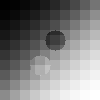
\includegraphics[width=35mm]{use-examples/pointmatching/mosaic-10-00-00.png} &
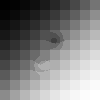
\includegraphics[width=35mm]{use-examples/pointmatching/mosaic-00-10-00.png} &
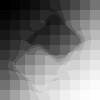
\includegraphics[width=35mm]{use-examples/pointmatching/mosaic-00-00-05.png} \\
$(d_p, d_f, \sigma_f) = (10,0,0)$ &
$(d_p, d_f, \sigma_f) = (0,10,0)$ &
$(d_p, d_f, \sigma_f) = (0,0,5)$ 
\end{tabular}
\end{center}
\caption{\label{fig:exe:pointmatching:2} Vector field deformation computation with only one non-null parameter.}
\end{figure}

On figure \ref{fig:exe:pointmatching:2}, it can be seen that deformations calculated with only one non-null parameter among $(d_p, d_f, \sigma_f)$ lead to non-homotopic deformations. Note that using only $\sigma_f$ should act as pure propagation (except at Vorono\"i diagram borders), but due to numerical reasons, the deformation becomes null when gaussian weights are too small.

\begin{figure}[ht]
\begin{center}
\begin{tabular}{ccc}
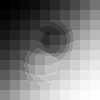
\includegraphics[width=35mm]{use-examples/pointmatching/mosaic-10-10-00.png} &
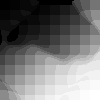
\includegraphics[width=35mm]{use-examples/pointmatching/mosaic-10-00-05.png} &
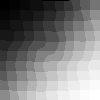
\includegraphics[width=35mm]{use-examples/pointmatching/mosaic-00-10-05.png} \\
$(d_p, d_f, \sigma_f) = (10,10,0)$ &
$(d_p, d_f, \sigma_f) = (10,0,5)$ &
$(d_p, d_f, \sigma_f) = (0,10,5)$ 
\end{tabular}
\end{center}
\caption{\label{fig:exe:pointmatching:3} Vector field deformation computation with only one null parameter.}
\end{figure}

Using two non-null parameters (see figure \ref{fig:exe:pointmatching:3}) allows to get continuous deformations: e.g., $(d_p, d_f, \sigma_f) = (10,0,5)$ and $(d_p, d_f, \sigma_f) = (0,10,5)$. However, deformations may be large at the Vorono\"i diagram borders ($(d_p, d_f, \sigma_f) = (10,0,5)$) or resulting deformations may be quite far away the desired ones ($(d_p, d_f, \sigma_f) = (10,0,5)$). 

Using all the three parameters may yield a deformation close to the expected one (see figure \ref{fig:exe:pointmatching:1}, left). 










\section{\applyTrsf and \blockmatching}
\label{sec:example:applyTrsf:blockmatching}

We exemplified here how to compute a transformation at a lower resolution (also described in section \ref{sec:hand:made:hierarchical:registration}) while still getting a deformed floating image at full resolution. Since the registration computation is done at a lower resolution, it is obviously faster (as it will be by tuning the \option{-pyramid-lowest-level}), but it also requires a little less computer memory. Such an approach can be used to tune parameters for instance.

Input images are of dimensions $481 \times 481$ with a pixel size of 0.5 image (see figure \ref{fig:exe:applyTrsf:blockmatching:1}). They can be non-linearly registered through (registration result can be seen in figure \ref{fig:exe:applyTrsf:blockmatching:1}, middle)
\begin{code}{1}
\% blockmatching -ref ref.mha -flo flo.mha -res res.mha -trsf-type vectorfield -res-trsf vector.trsf -elastic-sigma 2.5 -fluid-sigma 1.0
\end{code}
Options \option{-elastic-sigma 2.5 -fluid-sigma 1.0} have been chosen to enhance deformations.

\begin{figure}[ht]
\begin{center}
\begin{tabular}{ccc}
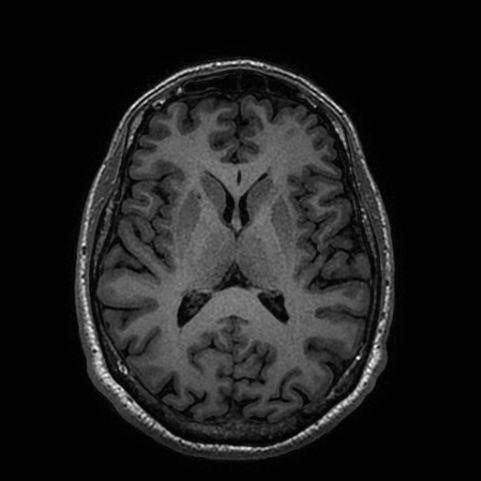
\includegraphics[width=35mm]{use-examples/applyTrsf-blockmatching/ref.png} &
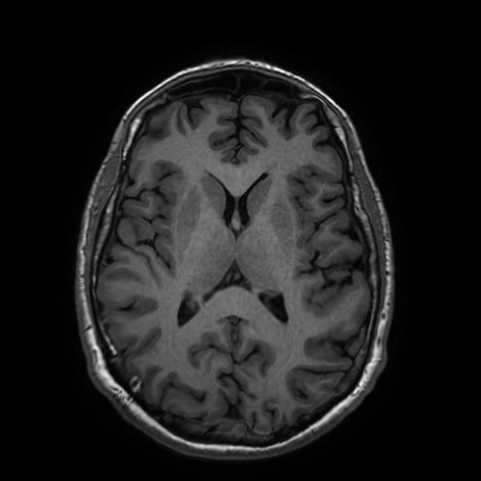
\includegraphics[width=35mm]{use-examples/applyTrsf-blockmatching/res.png} & 
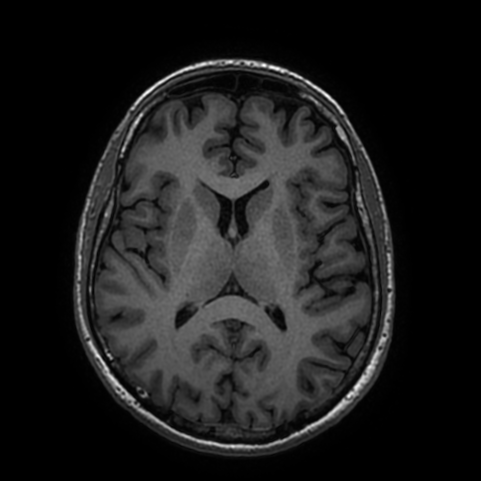
\includegraphics[width=35mm]{use-examples/applyTrsf-blockmatching/flo.png} \\
Reference image &
High resolution result &
Floating image \\
& (deformed floating image) &
\end{tabular}
\end{center}
\caption{\label{fig:exe:applyTrsf:blockmatching:1} Input images for registration. Please notice the smaller ventricles of the floating image. Images dimensions are $481 \times 481$.}
\end{figure}

Input images are downsampled with the following commands (see figure \ref{fig:exe:applyTrsf:blockmatching:2}). Note that, even here the commands are similar, they could have been resampled at different resolutions.
\begin{code}{1}
\% applyTrsf flo.mha lower-flo.mha -iso 2.0 -resize -res-trsf lower-flo.trsf \\
\% applyTrsf ref.mha lower-ref.mha -iso 2.0 -resize -res-trsf lower-ref.trsf
\end{code}
Here images are downsampled to a pixel size of 2.0, yielding images of dimensions $120 \times 120$. These images can be non-linearly registered through  (registration result can be seen in figure \ref{fig:exe:applyTrsf:blockmatching:2}, middle)
\begin{code}{1}
\% blockmatching -ref lower-ref.mha -flo lower-flo.mha -res lower-res.mha -trsf-type vectorfield -res-trsf lower-vector.trsf -elastic-sigma 2.5 -fluid-sigma 1.0
\end{code}

\begin{figure}[ht]
\begin{center}
\begin{tabular}{ccc}
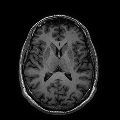
\includegraphics[width=35mm]{use-examples/applyTrsf-blockmatching/lower-ref.png} &
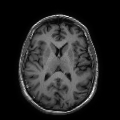
\includegraphics[width=35mm]{use-examples/applyTrsf-blockmatching/lower-res.png} &
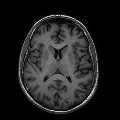
\includegraphics[width=35mm]{use-examples/applyTrsf-blockmatching/lower-flo.png} \\
Reference image &
Low resolution result &
Floating image \\
& (deformed floating image) &
\end{tabular}
\end{center}
\caption{\label{fig:exe:applyTrsf:blockmatching:2} Downsampled images and registration result. Images dimensions are $160 \times 160$.}
\end{figure}

To get the registration result at the original resolution, there are different possibilities.
\begin{enumerate}

\item The low resolution registration result can be upsampled in the same geometry than the reference image. To that end, the downsampling matrix (of the reference image) has first to be inverted. Then, the  low resolution registration result is resampled with this inverted transformation. It can be achieved with
\begin{code}{1}
\% invTrsf lower-ref.trsf inv-lower-ref.trsf \\
\% applyTrsf lower-res.mha resampled-lower-res.mha -trsf inv-lower-ref.trsf -template ref.mha
\end{code}
\begin{figure}[ht]
\begin{center}
\begin{tabular}{ccc}
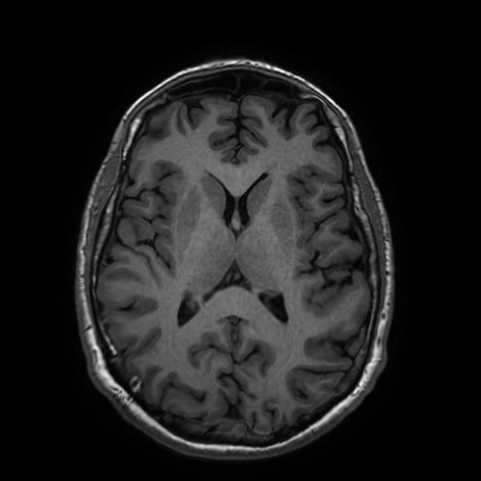
\includegraphics[width=35mm]{use-examples/applyTrsf-blockmatching/res.png} &
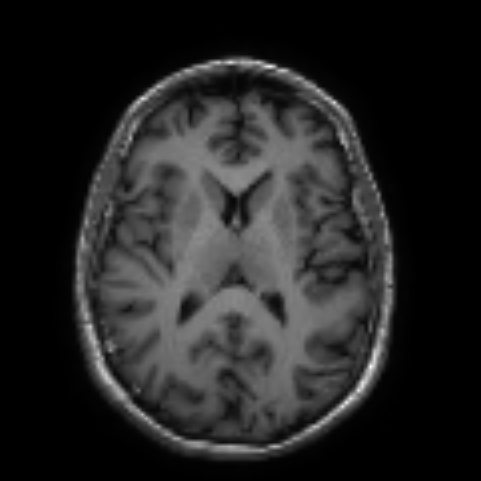
\includegraphics[width=35mm]{use-examples/applyTrsf-blockmatching/resampled-lower-res.png} &
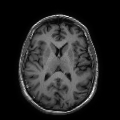
\includegraphics[width=35mm]{use-examples/applyTrsf-blockmatching/lower-res.png} \\
High resolution result &
Upsampled low resolution result &
Low resolution result \\
$481 \times 481$ &
$481 \times 481$ &
$160 \times 160$
\end{tabular}
\end{center}
\caption{\label{fig:exe:applyTrsf:blockmatching:3} Upsampling the low resolution registration result.}
\end{figure}
However, even though the upsampled low resolution registration result is of dimensions $481 \times 481$ with a pixel size of 0.5, the downsampling is visually present (see figure \ref{fig:exe:applyTrsf:blockmatching:3}).

\item A deformation at the high resolution can be computed from the deformation at the low resolution. It comes to compose transformations (see section \ref{sec:hand:made:hierarchical:registration}). The floating image at the high resolution can be then resampled thanks to this transformation. It can be done thanks to
\begin{code}{1}
\% invTrsf lower-ref.trsf inv-lower-ref.trsf \\
\% composeTrsf resampled-lower-vector.trsf -trsfs lower-flo.trsf lower-vector.trsf inv-lower-ref.trsf -template ref.mha \\
\% applyTrsf flo.mha lower-trsf-res.mha -trsf resampled-lower-vector.trsf -template ref.mha
\end{code}
\begin{figure}[ht]
\begin{center}
\begin{tabular}{ccc}
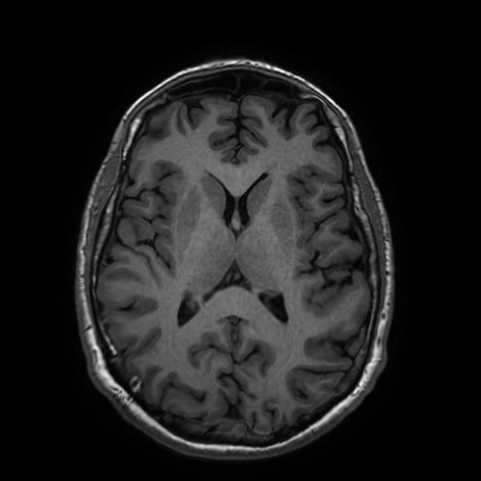
\includegraphics[width=35mm]{use-examples/applyTrsf-blockmatching/res.png} &
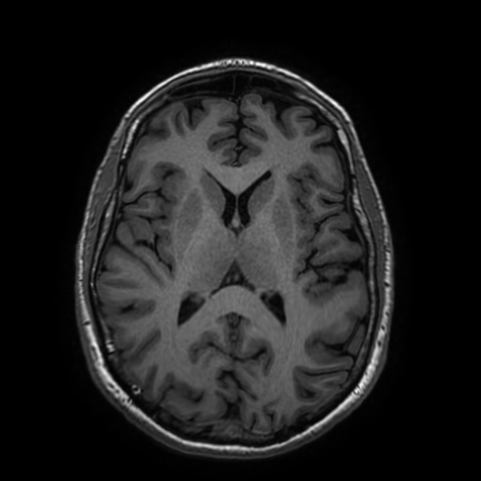
\includegraphics[width=35mm]{use-examples/applyTrsf-blockmatching/lower-trsf-res.png} &
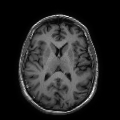
\includegraphics[width=35mm]{use-examples/applyTrsf-blockmatching/lower-res.png} \\
High resolution result &
High resolution result  &
Low resolution result \\
& from low resolution transformation & \\
$481 \times 481$ &
$481 \times 481$ &
$160 \times 160$
\end{tabular}
\end{center}
\caption{\label{fig:exe:applyTrsf:blockmatching:4} Upsampling the low resolution registration result.}
\end{figure}
The result can be see in figure \ref{fig:exe:applyTrsf:blockmatching:4}.

\end{enumerate}


